% !TeX spellcheck = en_US	


\documentclass[10pt,journal,compsoc]{IEEEtran}
\usepackage{graphicx}
\usepackage[ruled, linesnumbered]{algorithm2e}
\usepackage{url}
\usepackage{epstopdf}
\usepackage{indentfirst}
\usepackage[tight,footnotesize]{subfigure}
\usepackage{amsmath}
\usepackage{amssymb}
\usepackage{multirow}
\usepackage{color}
\usepackage{enumerate}

\newtheorem{Formula}{Formula}
\newtheorem{Lemma}{Lemma}
\newtheorem{Corollary}{Corollary}
\newtheorem{Property}{Property}
\newtheorem{Rule}{Rule}

% *** CITATION PACKAGES ***
\ifCLASSOPTIONcompsoc
\usepackage[nocompress]{cite}
\else
\usepackage{cite}
\fi


\begin{document}


\title{Checking Big Suffix and LCP Arrays by Probabilistic Methods}

\author{
	Yi~Wu,
	Ge~Nong,
	Wai~Hong~Chan,
	Ling~Bo~Han% <-this % stops a space
	\IEEEcompsocitemizethanks{
		\IEEEcompsocthanksitem Y. Wu, G. Nong (corresponding author) and L.~B.~Han are with the Department of Computer Science, Sun Yat-sen University, Guangzhou 510275, China. E-mails: wu.yi.christian@gmail.com, issng@mail.sysu.edu.cn, hanlb@mail2.sysu.edu.cn.
		
		\IEEEcompsocthanksitem Wai Hong Chan (corresponding author) is with the Department of Mathematics and Information Technology, The Education University of Hong Kong, Hong Kong. E-mail: waihchan@ied.edu.hk.
}}% <-this % stops a space
	
\IEEEtitleabstractindextext{%
\begin{abstract}

For full-text indexing of massive data, the suffix and LCP (longest common prefix) arrays have been recognized as the fundamental data structures, and there are at least two needs in practice for checking their correctness, i.e. program debugging and verifying the arrays constructed by probabilistic algorithms.
We propose in this paper two methods to check the suffix and LCP arrays in external memory by using a Karp-Rabin fingerprinting technique, where the checking result is wrong only with a negligible error probability. Our first method checks the lexicographical order and the LCP-value of two neighboring suffixes in the given suffix array by computing and comparing the fingerprints of their LCPs. This approach is also employed in the second method to verify a subset of the given suffix and LCP arrays, from which then a copy of the final suffix and LCP arrays is produced following the induced sorting principle and compared with the given one for verification.


\end{abstract}

% Note that keywords are not normally used for peerreview papers.
\begin{IEEEkeywords}
	Suffix and LCP arrays verification, Karp-Rabin fingerprinting technique, external memory.
\end{IEEEkeywords}}


% make the title area
\maketitle

\IEEEdisplaynontitleabstractindextext

\IEEEpeerreviewmaketitle

\section{Introduction}\label{sec:introduction}

\subsection{Background} \label{sec:introduction:background}


Suffix and longest common prefix (LCP) arrays play an important role in various string processing tasks, such as data compression, pattern matching and genome assembly. Particularly, these two data structures constitute the core part of a powerful full-text index, called enhanced suffix array~\cite{Abouelhodaa2004}, which is more space efficient than suffix tree and applicable to emulating any searching functionalities provided by the latter in the same time complexity. The first algorithm for building SA in internal memory was presented in~\cite{Manber1993}. From then on, much effort has been put on the development of designing efficient SA construction algorithms~(SACAs) on different computation models, e.g., internal memory~\cite{Karkkainen2003, Ko2003, Kim2003, Nong11}, external memory~\cite{Dementiev2008, Ferragina2012, Manzini2004, Bingmann12, Karkkainen2014, Nong14, Nong15} and shared memory models~\cite{Osipov2012, Deo2013, Wang2015, Karkkainen2015}. In respect of the design on LCP-array construction algorithms~(LACAs), the existing works can be classified into two categories, where the algorithms of the first category compute the suffix and LCP arrays in the same time~\cite{Fischer11, Bingmann12, Flick2015} and that of the second category take the suffix array (SA) and/or Burrows-Wheeler transform (BWT) as input to facilitate the computation~\cite{Kasai2001,Karkkainen2009, Fischer11, Puglisi2008, Puglisi2008, Deo2013, Karkkainen2016}. Currently, the fastest algorithms of linear time and space complexity are based on induced sorting principle. However, some sub-linear algorithms reported recently achieved a better performance by exploiting the full use of computation resource in a multi-core environment.
 

{\color{red} There are at least two needs in practice for checking the correctness of a suffix or LCP array, i.e. program debugging and verifying the array constructed by a probabilistic algorithm.}
While the study for efficient construction of suffix and LCP arrays is evolving, the programs implementing the proposed algorithms are commonly provided ``as is", with the purpose only for the performance evaluation experiemnts of the articles where they are reported. That is, these programms give no guarantee that they have correctly implemented the proposed algorithms. The programs for recently proprosed algorithms are becoming much more complicated than before, casuing {\color{red} challenges} for program verifying and debugging\footnote{In our studies before, we have exprienced problems caused by bugs of the exisitng programs.}. As a common practice, a suffix or LCP array checker is also provided for verifying the correctness of a constructed array. For example, such a checker is provided in the software packages (like SA-IS~\cite{Nong11}, eSAIS~\cite{Bingmann12} and DC3~\cite{Dementiev08}) for constructing suffix and/or LCP arrays. In addition to help avoid implementation bugs, a checker is also demanded for an array constructed by a probabilistic algorithm~\cite{Bille2013}. In this case, the array is correct with a probability and hence must be verified by a checker to ensure its correctness.

As far as we know, the work presented in~\cite{Burkhardt2003} is the only SA checking method that can be found in the existing literature, and no efficient approach for the LCP-array verification has been reported yet. In particular, there is currently no reported solution that can check both the suffix and the LCP arrays in external memory. This motivates our work here to design efficient external memory algorithms for checking the suffix and LCP arrays of massive data.
	
\subsection{Contribution}\label{sec:introduction:contribution}

Our contribution includes two checking methods for the given suffix and LCP arrays in external memory.

The main idea of the first method is to test the lexical order and the LCP-value of two neighboring suffixes in a suffix array by literally comparing their characters. To reduce time complexity for a comparison between two sequences of characters, a Karp-Rabin fingerprinting function is employed to transform each sequence into a single integer, called fingerprint, such that the equality of two sequences can be correctly checked with a negiligible error probability by comparing their fingerprints in constant time.

By using the same fingerprinting technique, the second method first verifies a subset chosen from the input arrays and then produces a copy of the suffix and LCP arrays from the verified subset following the induced sorting~(IS) principle. Given that the inducing process is correct, the input arrays are considered to be right with a high probability if they are equal to the induced copies.

The remainder of this paper is organized as follows. We first describe the proposed two checking methods in Sections~\ref{sec:method1} and~\ref{sec:method2}, then present the experimental results in Section~\ref{sec:experiment},and give the conclusion in Section~\ref{sec:conclusion}.


\section{Method A} \label{sec:method1}


\subsection{Preliminaries} \label{sec:method1:notations}

Given an input string $x[0, n)$ drawn from an alphabet $\Sigma$, the suffix array of $x$, denoted by $sa$, is a permutation of $\{0, 1, ..., n - 1\}$ such that ${\sf suf}(sa[i]) < {\sf suf}(sa[j])$ is satisfied for $0 \le i < j < n$, where ${\sf suf}(sa[i])$ and ${\sf suf}(sa[j])$ are two suffixes starting with $x[sa[i]]$ and $x[sa[j]]$, respectively. Particularly, we say ${\sf suf}(sa[i - 1])$ and  ${\sf suf}(sa[i + 1])$ are the lexical neighbors of ${\sf suf}(sa[i])$ in $sa$. The LCP array of $x$, denoted by $lcp$, consists of $n$ integers, where $lcp[0]:=0$ and $lcp[i]$ records the LCP-value of ${\sf suf}(sa[i])$ and ${\sf suf}(sa[i - 1])$ for $i \in [1, n)$.


\subsection{Idea} \label{sec:method1:idea}

The lexical order and the LCP-value of ${\sf suf}(sa[i])$ and ${\sf suf}(sa[j])$ can be determined by literally comparing their characters from left to right. Because all the suffixes differ in length and end with a common character, there must exist $k \in [0, n)$ such that $x[i, i + k) = x[j, j + k)$ and $x[i + k] \ne x[j + k]$. According to Lemma~\ref{lemma:1}, this method can be also applied to checking suffix and LCP arrays, but it suffers from high time complexity as the two substrings indicated by the LCP-value for each pair of neighboring suffixes in $sa$ take at worst $\mathcal{O}(n)$ character-wise comparisons.

\begin{Lemma} \label{lemma:1}
	Both $sa[0, n)$ and $lcp[0, n)$ are correct if and only if the following conditions are satisfied, for all $i \in [1, n)$:
	\begin{enumerate}[(1)]
		\item
		$sa$ is a permutation of $\{0, 1, \dots, n - 1\}$.
		\item
		$x[sa[i], sa[i] + lcp[i] - 1] = x[sa[i - 1], sa[i - 1] + lcp[i] - 1]$.
		\item
		$x[sa[i] + lcp[i]] > x[sa[i - 1] + lcp[i]]$. 	
	\end{enumerate}
\end{Lemma}

\begin{IEEEproof}
	Both the sufficiency and necessity are immediately seen from the definition of suffix and LCP arrays. Specifically, condition (1) demonstrates that all the suffixes in $x$ are sorted in $sa$, while conditions (2)-(3) indicate that the lexical order and the LCP-value of any two neighboring suffixes in $sa$ are both correct.
\end{IEEEproof}

An alternative is to exploit a perfect hash function~(PHF) to convert each substring into a single integer such that any two substrings have a common hash value if and only if they are literally equal to each other. Hence, the equality of two substrings can be determined by comparing the corresponding hash values instead. The key point here is how to efficiently compute the hash values of $x[sa[i], sa[i] + lcp[i] - 1]$ and $x[sa[i - 1], sa[i - 1] + lcp[i] - 1]$ for all $i \in [1, n)$. Taking into account the high cost of finding a PHF to meet this requirement, we prefer using a Karp-Rabin fingerprinting function~\cite{Karp1987} to transform a substring into its integer form, called fingerprint. Specifically, suppose $L$ is a prime and $\delta$ is randomly chosen from $[1, L)$, the fingerprint ${\sf fp}(i, j)$ of a substring $x[i, j]$ can be calculated by using Formulas~\ref{formula:1}-~\ref{formula:3} as following: scan $x$ rightward to iteratively compute ${\sf fp}(0, k)$ for all $k \in [0, n)$ according to Formulas~\ref{formula:1}-\ref{formula:2}, meanwhile, record ${\sf fp}(0, i - 1)$ and ${\sf fp}(0, j)$ and subtract the former from the latter to obtain ${\sf fp}(i, j)$ according to Formula~\ref{formula:3}.

\begin{Formula} \label{formula:1}
	${\sf fp}(0, -1) = 0$.
	
\end{Formula}

\begin{Formula} \label{formula:2}	
	${\sf fp}(0, i) = {\sf fp}(0, i - 1) \cdot {\delta} + x[i]\mod L$ for $i \ge 0$.
	
\end{Formula}

\begin{Formula} \label{formula:3}
	${\sf fp}(i, j) = {\sf fp}(0, j) - {\sf fp}(0 ,i - 1) \cdot {\delta}^{j - i + 1}\mod L$.
	
\end{Formula}

It is worthy of mentioning that two equal substrings always share a common fingerprint, but the inverse is not true. Fortunately, it has been proved in~\cite{Karp1987} that the probability of a false match can be reduced to a negligible level by setting $L$ to a large value\footnote{This property is utilized in~\cite{Bille2013} to design a probabilistic algorithm for computing a sparse suffix array. }. This leads us to the following conclusion.

\begin{Corollary} \label{corollary:1}
	Both $sa[0, n)$ and $lcp[0, n)$ are correct with a high probability given the following conditions, for all $i \in [1, n)$:
	
	\begin{enumerate}[(1)]
		\item
		$sa$ is a permutation of $\{0, 1, \dots, n - 1\}$.
		
		\item
		${\sf fp}(sa[i], sa[i] + lcp[i] - 1) = {\sf fp}(sa[i - 1], sa[i - 1] + lcp[i] - 1)$.
		
		\item
		$x[sa[i] + lcp[i]] > x[sa[i - 1] + lcp[i]]$.
	\end{enumerate}
\end{Corollary}


\subsection{Algorithm} \label{sec:method1:algorithm}

Section~\ref{sec:method1:idea} indicates that we can perform verification for the given suffix and LCP arrays by testing the conditions of Corollary~\ref{corollary:1}. Based on this idea, we introduce below a linear algorithm for checking $sa$ and $lcp$ on random access models.

\begin{enumerate}
	\item [S1]
	Scan $x$ rightward with $i$ increasing from $0$ to $n - 1$. For each scanned $x[i]$, iteratively compute ${\sf fp}(0, i)$ and set $fp[i] = {\sf fp}(0, i)$.
	
	\item [S2]
	Scan $sa$ and $lcp$ rightward with $i$ increasing from $1$ to $n - 1$. For each scanned $sa[i]$ and $lcp[i]$, let $u = sa[i], v = lcp[i], w = sa[i - 1]$ and performs substeps (a)-(c) sequentially:
	
	\begin{enumerate}[(a)]
		\item
		Retrieve $fp[u - 1]$ and $fp[u + v - 1]$ from $fp$ to compute ${\sf fp}(u, u + v - 1)$. Set $mk[u] = 1$.
		
		\item
		Retrieve $fp[w - 1]$ and $fp[w + v - 1]$ from $fp$ to compute ${\sf fp}(w, w + v - 1)$.
		
		\item
		Check if ${\sf fp}(u, u + v - 1) = {\sf fp}(w, w + v - 1)$ and $x[u + v] > x[w + v]$.
		
		\item
		Set $mk[sa[0]] = 1$.
	\end{enumerate}

	\item [S3] Check if $mk[i] = 1$ for all $i \in [0, n)$.
	
\end{enumerate}

Two zero-initialized arrays $fp$ and $mk$ are used to faciliate the checking process, where the former is for storing the fingerprints of all the prefixes in $x$ and the latter is for checking the existence of $\{0, 1, ..., n - 1\}$ in $sa$. Assume $L = 197$ and $\delta = 101$, we give a small example of S1-S2 in Fig.~\ref{fig:example} for better understanding. Clearly, this algorithm consumes $\mathcal{O}(n)$ time and space when running in internal memory. However, if the input can not be wholly accommodated into RAM, it may suffer from a performance degradation due to frequent random I/O operations for reading elements of $x$, $sa$ and $lcp$ from external memory during the execution of S2.

\begin{figure*}
	\centering
	\label{fig:example}
	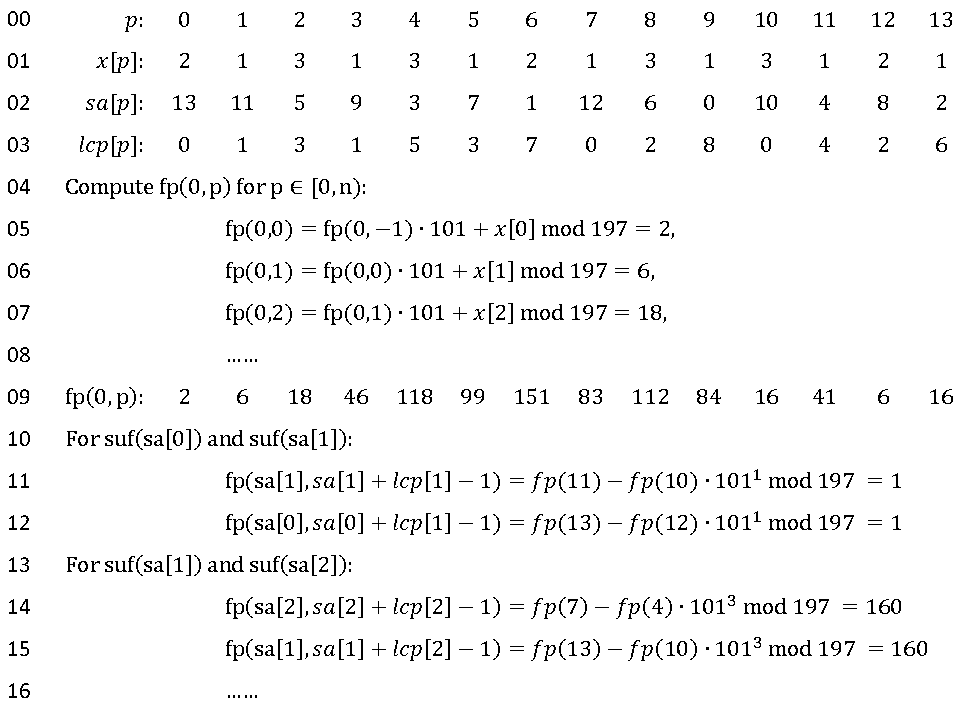
\includegraphics[width = 0.8\textwidth]{example}
	\caption{An Example for Checking the Suffix and LCP Arrays Using the Karp-Rabin Fingerprinting Functions}	
\end{figure*}

\SetKwProg{Fn}{Function}{}{}

\begin{algorithm*}

	\caption{The Algorithm for checking the conditions of Corollary~\ref{corollary:1}.}
	
	\label{alg:1}
	
	%\SetAlgoNoLine
	\Fn{{\sf CheckByFP}($x$, $sa$, $lcp$, $n$)}{
	
		$ST_1$ := $[(sa[i], i, null) | i \in [0, n)]$. \label{alg:1:a}
		
		$ST_2$ := $[(sa[i] + lcp[i + 1], i, null, null) | i \in [0, n - 1)]$.
			
		$ST_3$ := $[(sa[i] + lcp[i], i, null, null) | i \in [1, n)]$.
		
		sort tuples in $ST_1$, $ST_2$ and $ST_3$ by 1st component. \label{alg:1:b}
		
		$fp := 0$  \label{alg:1:c}
		
		\For{$i \in [0, n]$}{
			
			\If{$ST_1.{\sf notEmpty}()$ {\sf and} $ST_1.{\sf top}().1st = i$}{~\label{alg:1:h}
				$e := ST_1.{\sf top}()$, $ST_1.{\sf pop}()$, $e.3rd := fp$, $ST_1'.{\sf push}(e)$
			}
			\Else{
				\Return false \hspace{5cm} // condition (1) is violated
			}~\label{alg:1:i}
			\While{$ST_2.{\sf notEmpty}()$ {\sf and} $ST_2.{\sf top}().1st = i$}{
				
				$e := ST_2.{\sf top}()$, $ST_2.{\sf pop}()$, $e.3rd := fp$, $e.4th := x[i]$, $ST_2'.{\sf push}(e)$
			}	
		
			\While{$ST_3.{\sf notEmpty}()$ {\sf and} $ST_3.{\sf top}().1st = i$}{
				
				$e := ST_3.{\sf top}()$, $ST_3.{\sf pop}()$, $e.3rd := fp$, $e.4th := x[i]$, $ST_3'.{\sf push}(e)$
			}	
		
			$fp := fp \cdot \delta + x[i] \! \mod \! P$
		} \label{alg:1:d}
		
		sort tuples in $ST_1$, $ST_2$ and $ST_3$ by 2nd component.  \label{alg:1:e}
		
		\For {$i \in [1, n - 1)$}{  \label{alg:1:f}
			
			$fp_1 := ST_1'.{\sf top}().3rd$, $ST_1'.{\sf pop}()$, $fp_2 := ST_2'.{\sf top}().3rd$, $ch_1 := ST_2'.{\sf top}().4th$, $ST_2'.{\sf pop}()$
			
			$\hat{fp_1} = fp2 - fp1 \cdot \delta^{lcp[i]} \! \mod \! P$ \label{alg:1:j}
		
		 	$fp_1 := ST_1'.{\sf top}().3rd$, $fp_3 := ST_2'.{\sf top}().3rd$, $ch_2 := ST_3'.{\sf top}().4th$, $ST_3'.{\sf pop}()$
			
			$\hat{fp_2} = fp3 - fp1 \cdot \delta^{lcp[i]} \! \mod \! P$	\label{alg:1:k}
			
			\If{$\hat{fp_1} \ne \hat{fp_2}$ {\sf or} $ch_1 \le ch_2$}{
				
				\Return false \hspace{5cm} // condition (2) or (3) is violated
			}	
		} \label{alg:1:g}

		\Return true
	}
\end{algorithm*}


We propose Algorithm~\ref{alg:1} to perform the checking process in an I/O friendly way, which conducts external-memory sorts to avoid random accesses to external disks.
At the very beginning, the algorithm first scans $sa$ and $lcp$ to produce $ST_1, ST_2, ST_3$ and sorts the tuples of them by 1st component in ascending order (lines~\ref{alg:1:a}-\ref{alg:1:b}).
Then, it computes the fingerprints of all the prefixes according to Formulas~\ref{formula:1}-\ref{formula:2} and assign them to the sorted tuples in lines~\ref{alg:1:c}-\ref{alg:1:d} as following: when finished computing ${\sf fp}(0, i - 1)$, extract each tuple $e$ with $e.1st = i$ from $ST_1, ST_2, ST_3$  and update them with ${\sf fp}(0, i - 1)$ and $x[i]$ (if required), where the tuples are forwarded to $ST_1', ST_2', ST_3'$ after updating and sorted back to their original order (line~\ref{alg:1:e}).
During the process, we determine whether or not the 1st components of all the tuples in $ST_1$ consistute a permutation of $\{0, 1, ..., n - 1\}$ to test the first condition of Corollary~\ref{corollary:1} (lines~\ref{alg:1:h}-\ref{alg:1:i}).
Finally, it repeatedly retrieves the top tuples from $ST_1', ST_2', ST_3'$ and applies Formulas~\ref{formula:3} to compute the fingerprints of two substrings specified by their 1st components for ensuring the satisfaction of conditions (2)-(3). A point to be explained here is how to compute $\delta^{lcp[i]}$ in lines~\ref{alg:1:j} and~\ref{alg:1:k}. Let $e := lcp[i]$, our method first decomposes $e$ into $\Sigma_{i = 0}^{\lceil \log2^n \rceil}{k_i \cdot 2^i}$ and then computes $\Pi_{i = 0}^{\lceil \log2^n \rceil}{\delta}^{k_i \cdot 2^i}$ to obtain $\delta^{e}$, where $k_i \in \{0, 1\}$. Following this way, the answer can be returned in $\mathcal{O}(\lceil \log2^n \rceil)$ time using $\mathcal{O}(\lceil \log2^n \rceil)$ space for storing $\{{\delta}^{1}, {\delta}^{2}, \dots, {\delta}^{2^{\lceil \log2^n \rceil}} \}$.

\subsection{Discussion} \label{sec:method1:discussion}

Algorithm~\ref{alg:1} performs multiple scans and sorts for arrays of $n$ fixed-size tuples using external memory. Consider an external memory model with RAM size $M$, disk size $D$ and block size $B$, all are in words, then the time and I/O complexities for a scan are $\mathcal{O}(n)$ and $\mathcal{O}(n / B)$, respectively, while those for a sort with an integer key are $\mathcal{O}(n\log_{M/ B}(n / B))$ and $\mathcal{O}((n / B)\log_{M / B}(n / B))$, respectively~\cite{Arge2013}. Besides, the algorithm reaches its peak disk use when sorting tuples in lines~\ref{alg:1:b} and~\ref{alg:1:e}. An optimization for reducing maximum space requirements is to compute the fingeprints indicated by $ST_1, ST_2, ST_3$ separately. This will lead to a small increase in total I/O volume as it needs to compute $\{{\sf fp}(0, 0), {\sf fp}(0, 1), ..., {\sf fp}(0, n - 1)\}$ two more times.
	
	

\section{Method B} \label{sec:method2}

Our experimental study in Section~\ref{sec:experiment} shows that Algorithm~\ref{alg:1} is quite space consuming, its peak disk use is 40 bytes per input character. In this section, we describe an alternative based on the induced-sorting principle. Compared with Algorithm~\ref{alg:1}, the algorithm designed by this method only takes half space on real-world datasets.

\subsection{Preliminaries} \label{sec:method2:preliminaries}

Before our presentation, we first introduce some notations for description convenience.

{\em Character and suffix classification.} All the characters in $x$ are classified into three types, namely L-, S- and S*-type. Detailedly, $x[i]$ is L-type if (1) $i = n - 1$ or (2) $x[i] > x[i + 1]$ or (3) $x[i] = x[i + 1]$ and $x[i + 1]$ is L-type; otherwise, $x[i]$ is S-type. Further, if $x[i]$ and $x[i + 1]$ are S- and L-type respectively, then $x[i]$ is also an S*-type character. Moreover, the type of a suffix is the same as that of its heading character.

{\em Suffix and LCP buckets.} Suppose $sa$ is correct, then suffixes in $sa$ are naturally partitioned into multiple buckets and those with an identical heading character are grouped into one bucket occupying a contiguous interval. Further, a bucket can be divided into two parts, where the left and right part contain L- and S-type suffixes, respectively. For short, we use ${\sf sa\_bkt}(c)$ to denote the bucket storing suffixes starting with $c$ and ${\sf sa\_bkt_L}(c)/{\sf sa\_bkt_S}(c)$ to denote its left/right sub-bucket. Accordingly, $lcp$ can be decomposed into multiple buckets as well, where ${\sf lcp\_bkt}(c)/{\sf lcp\_bkt_L}(c)/{\sf lcp\_bkt_S}(c)$ store the LCP-values of suffixes in ${\sf sa\_bkt}(c)/{\sf sa\_bkt_L}(c)/{\sf sa\_bkt_S}(c)$ and their left lexical neighbors.

{\em Suffix and LCP arrays for S*-type suffixes.} Suppose the number of S*-type suffixes in $x$ is $n_1$, $sa^*[0, n_1)$ and $lcp^*[0, n_1)$ indicate the lexical order and the LCP-values of these S*-type suffixes, where $x[sa^*[i]]$ is the heading character of the $(i + 1)$-th smallest S*-type suffix.

{\em Type array.} The type array $t$ records the type of $x[i]$ in $t[i]$ for $i \in [0, n)$.

\subsection{Idea} \label{sec:method2:idea}

The induced sorting principle has been employed to design algorithms for constructing suffix and LCP arrays in both internal and external memory. These algorithms mainly consist of a reduction phase for computing $sa^*$ and $lcp^*$ followed by an induction phase for inducing $sa$ and $lcp$ from $sa^*$ and $lcp^*$. Suppose $sa^*$ and $lcp^*$ are already known, we can directly build the suffix and LCP arrays by calling the inducing process of an existing IS-based construction algorithm. This enlightens us to check the following conditions for verification:
	
\begin{Lemma} \label{lemma:2}
Both $sa[0, n)$ and $lcp[0, n)$ are correct if and only if the conditions below are satisfied:

\begin{enumerate}[(1)]
	\item
	$sa^*$ and $lcp^*$ are both correct.
	\item
	$sa = sa'$ and $lcp = lcp'$, where $sa'$ and $lcp'$ are induced from $sa^*$ and $lcp^*$ by calling the inducing process of an existing IS-based construction algorithm.
\end{enumerate}
\end{Lemma}

Following the same idea described in Section~\ref{sec:method1:idea}, we come to the conclusion in Corollary~\ref{corollary:2} by using the fingerprinting technique.

\begin{Corollary} \label{corollary:2}
Both $sa[0, n)$ and $lcp[0, n)$ are correct with a high probability given the following conditions, for $i \in [0, n)$, $j, k \in [1, n_1)$ and $j \ne k$:
	
\begin{enumerate}[(1)]
	\item
	$sa^*[j] \ne sa^*[k]$.
	\item
	${\sf fp}(sa^*[j], sa^*[j] + lcp^*[j] - 1) = {\sf fp}(sa^*[j - 1], sa^*[j - 1] + lcp^*[j] - 1)$.
	\item
	$x[sa^*[j] + lcp^*[j]] > x[sa^*[j - 1] + lcp^*[j]]$.
	\item
	$sa[i] = sa'[i]$ and $lcp[i] = lcp'[i]$, where $sa'$ and $lcp'$ are induced from $sa^*$ and $lcp^*$ by calling the inducing process of an existing IS-based construction algorithm.
\end{enumerate}

\end{Corollary}


\subsection{Algorithm} \label{sec:method2:algorithm}
Algorithm~\ref{alg:2} checks the conditions in Corollary~\ref{corollary:2} using external memory, the details are shown as following. The first task of the algorithm is to retrieve $sa^*$ and $lcp^*$ from $sa$ and $lcp$. For the purpose, it creates a tuple for each suffix in $sa$ and sorts them by 1st component in descending order~(lines~\ref{alg:2:a}-\ref{alg:2:b}). After sorting, it scans $x$ leftward to find all the S*-type suffixes according to the definition in Section~\ref{sec:method2:preliminaries}~(lines~\ref{alg:2:c}-\ref{alg:2:d}). For each S*-type suffix, we pick the corresponding tuple from the top of $ST_1$ and forward the tuple to $ST_2$. Then, the algorithm sorts $ST_2$ by 2nd component in ascending order and scans the sorted tuples sequentially to produce $sa^*$ and $rank^*$, where $rank*$ is the compact form of $sa^*$. Meanwhile, we compute $lcp^*$ following the fact that the LCP-value of two suffixes in ${\sf suf}(sa[i])$ and ${\sf suf}(sa[j])$ ($i < j$) is the minimum value among $\{lcp[i + 1], ..., lcp[j - 1], lcp[j]\}$~(lines~\ref{alg:2:g}-\ref{alg:2:h}). The next task is to check the correctness of $sa^*$ and $lcp^*$. This is accomplished in lines~\ref{alg:2:i}-\ref{alg:2:j} by reusing Algorithm~\ref{alg:1}. At last, we call the inducing process of an external-memory construction algorithm to generate $sa'$ and $lcp'$~(line~\ref{alg:2:k}), and compare the output with $sa$ and $lcp$ to determine the result in lines~\ref{alg:2:l}-\ref{alg:2:m}.

\begin{algorithm*}
	
	\caption{The Algorithm for checking the conditions of Corollary~\ref{corollary:2}.}
	
	\label{alg:2}
	
	%\SetAlgoNoLine
	\Fn{{\sf CheckByIS}($x$, $sa$, $lcp$, $n$)}{	
	
	$ST_1$ := $[(sa[i], i, null) | i \in [0, n)]$ \label{alg:2:a}
		
	sort tuples in $ST_1$ by 1st component \label{alg:2:b}
	
	$r := 0$, $pos := -1$ \label{alg:2:c}
	
	\For{$i \in (n, 0]$}{
	
		$e := ST_1.{\sf top}()$, $ST_1.{\sf pop}()$
		
		\If{$x[i]$ is S*-type}{ \label{alg:2:e}
			
			\If{$pos \ge e.1st$}{
			
				\Return false  \hspace{1cm} // condition (1) is violated
			}
		
			$e.3rd := r$, $r := r + 1$, $ST_2.{\sf push}(e)$, $pos := e.1st$
		}\label{alg:2:f}
	} \label{alg:2:d}

	sort tuples in $ST_2$ by 2nd component \label{alg:2:g}
	
	$i := 0$, $j := 0$, $lcp_{min} := max\_val$
	
	\While{$ST_2.{\sf NotEmpty()}$}{
	
		$e := ST_2.{\sf top}()$, $ST_2.{\sf pop}()$
	
		\While {true} {
			
			$lcp_{min} := {\sf min}(lcp_{min}, lcp[i])$
			
			\If {$e.2nd = i$} {
			
				$sa^*[j] := e.1st$, $rank^*[j] := e.3rd$, $lcp^*[j] := lcp_{min}$, $j := j + 1$, $i:= i + 1$
				
				\textbf{break}
			}
			
			$i:= i + 1$
		}
	
		$lcp_{min} := max\_val$
	} \label{alg:2:h}
	
	\If{${\sf CheckByFP}(x, rank^*, lcp^*, lcp^*.{\sf size}()) = false$}{  \label{alg:2:i}
	
		\Return false;  \hspace{1cm} // conditions (2) or (3) is violated
	}\label{alg:2:j}

	$(sa', lcp') := {\sf InducingProcess}(x, sa^*, lcp^*)$ \label{alg:2:k}
	
	\For{$i \in [0, n)$}{\label{alg:2:l}
	
		\If{$sa[i] \ne sa'[i] \parallel lcp[i] \ne lcp'[i]$}{
		
			\Return false	// condition (4) is violated
		}	
	}\label{alg:2:m}

	\Return true
}
\end{algorithm*}

\subsection{Optimization} \label{sec:method2:optimization}

Algorithm~\ref{alg:2} produces a copy of the suffix and LCP arrays during the inducing process. Actually, given that $\Sigma$ is of a constant size, we can simply scan $sa/lcp$ to induce and check the suffixes/LCP arrays simultaneously without using extra space. The idea is that when a suffix/LCP-value $v_1$ is induced into a suffix/LCP bucket, we directly compare it with the corresponding item $v_2$ in $sa/lcp$. If $v_1 = v_2$, then $v_2$ is correct and can be used to induce subsequent suffixes/LCP-values. The key point here is how to retrieve elements from $sa/lcp$ quickly. This can be accomplished by conducting sequential I/O operations if we maintain a read pointer coupled with a buffer for each suffix/LCP sub-bucket. More details of the optimized inducing and checking processes as below, where $c \in [0, \Sigma)$ and $lp_1, lp_2, sp_1, sp_2$ are read pointer arrays for retrieving items from $sa/lcp$ buckets residing on disks.

\begin{enumerate}
	\item [S1]
	Let $lp_1[c]$ and $lp_2[c]$ point to the leftmost element of ${\sf sa\_bkt_L}(c)$ and ${\sf lcp\_bkt_L}(c)$ in $sa$ and $lcp$, respectively.
	\item [S2]
	Induce L-type suffixes and their LCP-values following the induced sorting principle. Meanwhile, for each induced L-type suffix $p$ with a heading character $c_0$ and its LCP-value $q$: (1) check $p = lp_1[c_0]$ and $q = lp_2[c_0]$; (2) let $lp_1[c_0]$ and $lp_2[c_0]$ point to the right neighbor in the same $sa$ and $lcp$ sub-buckets.
	\item [S3]
	Let $sp_1[c]$ and $sp_2[c]$ point to the rightmost element of ${\sf sa\_bkt_S}(c)$ and ${\sf lcp\_bkt_S}(c)$ in $sa$ and $lcp$, respectively.
	\item [S4]
	Induce S-type suffixes and their LCP-values following the induced sorting principle. Meanwhile, for each induced S-type suffix $p$ with a heading character $c_0$ and its LCP-value $q$: (1) check $p = sp_1[c_0]$ and $q = sp_2[c_0]$; (2) let $sp_1[c_0]$ and $sp_2[c_0]$ point to the left neighbor in the same $sa$ and $lcp$ sub-buckets.
\end{enumerate}


\subsection{Discussion} \label{sec:method2:discussion}

Both Algorithm~\ref{alg:2} and its optimized version can be implemented within sorting complexity. The space bottleneck occurs when inducing and checking the suffix and LCP arrays. This is because the existing IS-based construction algorithms store BWT to help retrieving preceding characters during the inducing process. We refer the interested readers to~\cite{Karkkainen2013} for more details.

\section{Experiments} \label{sec:experiment}

\subsection{Setup} \label{sec:experiment:setup}

The experimental platform is a work station equipped with an Intel Xeon E3-1220 V2 CPU, 4GiB RAM and 500GiB HD. To achieve high I/O efficiency, we implement the algorithms proposed in the previous sections using the external-memory containers provided by the STXXL library~\cite{Dementiev2007}. All the programs are compiled by gcc/g++ 4.8.4 with -O3 options under ubuntu 14.04 64-bit operating system. For performance analysis, we investigate on real-world datasets in Table~\ref{tbl:1} the following three metrics normalized by the size of input string:

\begin{itemize}
	
	\item RT: running time, in nanoseconds. Measured using the Linux 'time' command.
	
	\item PDU: peak disk use of external memory, in bytes.
	
	\item IOV: amount of data read from and write to external memory, in bytes.
	
\end{itemize}
	
%Table
\renewcommand\arraystretch{1.3}
\begin{table*}[!t]
	\caption{Corpus, $n$ in Gi, 1 byte per character}
	\label{tbl:1}
	\centering
	\begin{tabular}{|l|c|c|p{10cm}|}
		\hline
		Corpora & \multicolumn{1}{c|}{$n$} & \multicolumn{1}{c|}{$\|\Sigma\|$} & Description \\\hline
		enwiki & 8 & 256 & The 8-GiB prefix of an XML dump of English Wikipedia, available at \url{https://dumps.wikimedia.org/enwiki}, dated as 16/05/01. \\\hline	
		uniprot & 2.5 & 96 & UniProt Knowledgebase, available at \url{ftp://ftp.expasy.org/databases/.../complete}, dated as 16/05/11. \\\hline
		proteins & 1.1 & 27 & Swissprot database, available at \url{http://pizzachili.dcc.uchile.cl/texts/protein}, dated as 06/12/15. \\\hline
	\end{tabular}
\end{table*}

\subsection{Result} \label{sec:experiments:result}

Fig.~\ref{fig:cmp1} demonstrates the performance comparison between the programs for Algorithms~\ref{alg:1} and~\ref{alg:2}. As depicted,







The speed gap between them is mainly due to the difference in their I/O efficiencies. Specifically, the I/O volume of ProgB is 190$n$ in average, while that of ProgA is kept at 155$n$ for different corpora. Notice that, although Algorithm~\ref{alg:3} reuses Algorithm~\ref{alg:1} to check $sa_{\sf LMS}$ and $lcp_{\sf LMS}$, the consumption for the verification of $sa_{\sf LMS}$ and $lcp_{\sf LMS}$ in ProgB is at most half of ProgA because the number of LMS suffixes is no more than $\frac{1}{2}n$. It can be also observed that both programs are insensitive to the input corpus in terms of the space requirement. In details, the peak disk uses of ProgA and ProgB are respectively 26$n$ and 40$n$ on the three corpora.

We also investigate the performance trend of the two programs on the prefix of "enwiki" with the length varying on $\{1, 2, 4, 8\}$ GiB. Figure~\ref{fig:performance_analysis2} illustrates that, as the prefix length increases, a performance degradation occurs to ProgB in both time and I/O efficiencies, but the fluctuation of ProgA can be ignored.

%figure
\begin{figure}[htbp!]
	\centering
	\subfigure{
		\label{subfig:pdu_cmp}
		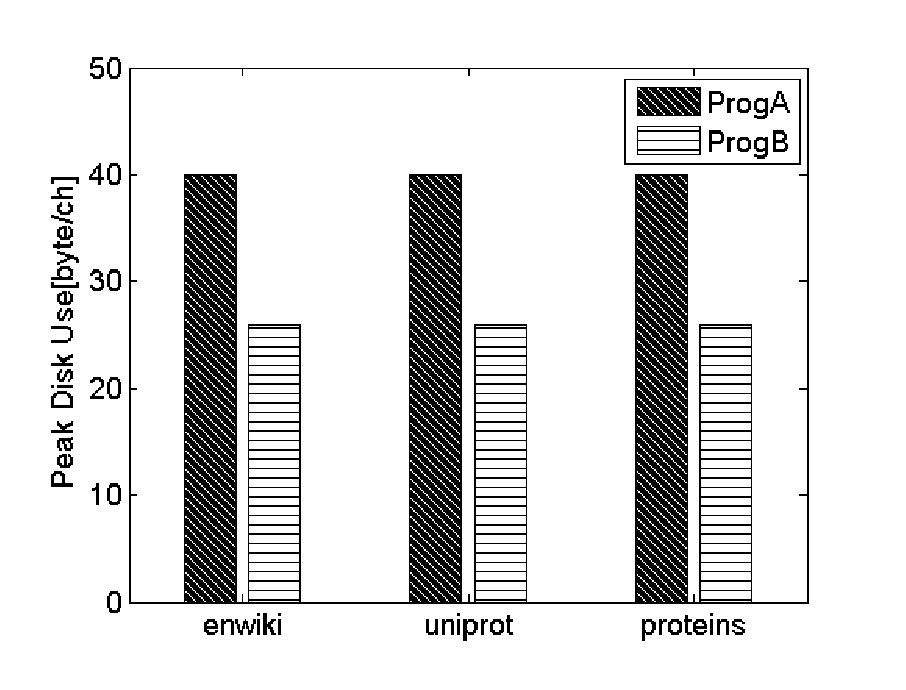
\includegraphics[width = 0.8\columnwidth]{pdu_cmp}
	}
	\hfil
	\subfigure{
		\label{subfig:iov_cmp}
		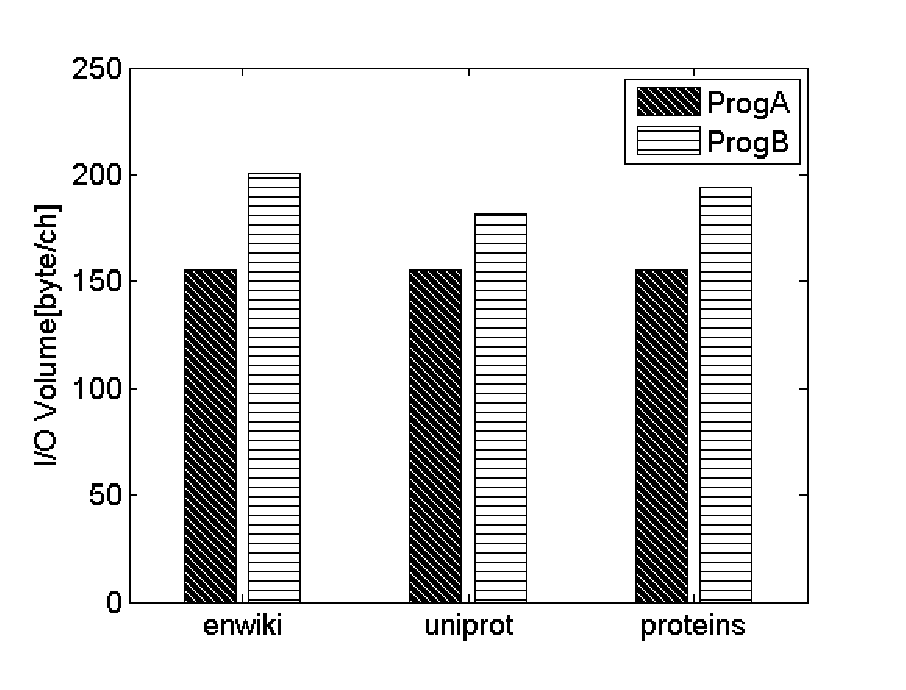
\includegraphics[width = 0.8\columnwidth]{io_cmp}
	}
	\hfil
	\subfigure{
		\label{subfig:ct_cmp}
		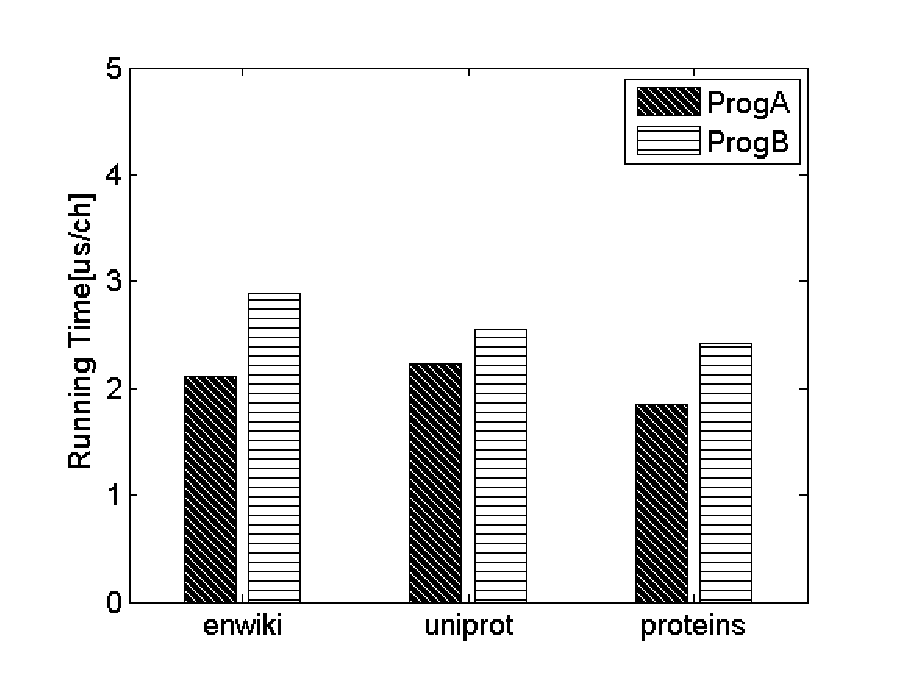
\includegraphics[width = 0.8\columnwidth]{ct_cmp}
	}
	\caption{Experimental results for various corpora.}
	\label{fig:performance_analysis}
\end{figure}

%figure
\begin{figure}[htbp!]
	\centering
	\subfigure{
		\label{subfig:pdu_cmp2}
		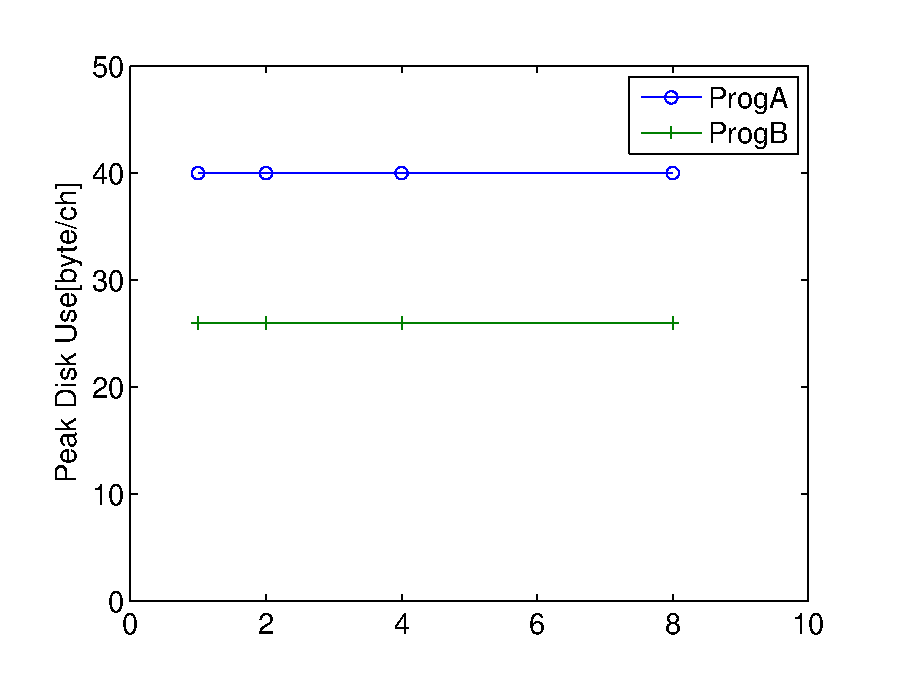
\includegraphics[width = 0.8\columnwidth]{pdu_cmp2}
	}
	\hfil
	\subfigure{
		\label{subfig:iov_cmp2}
		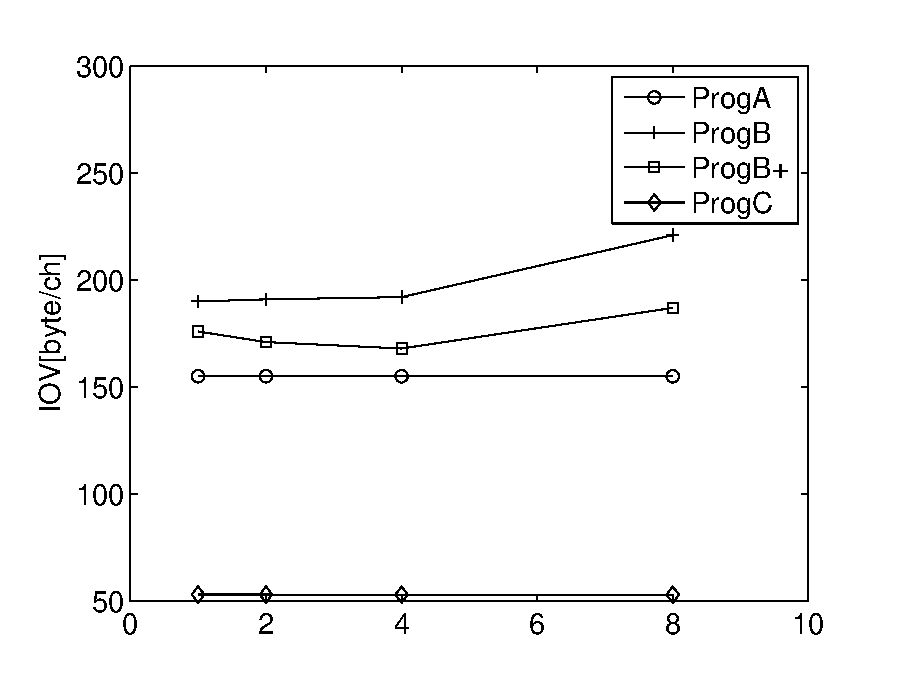
\includegraphics[width = 0.8\columnwidth]{io_cmp2}
	}
	\hfil
	\subfigure{
		\label{subfig:ct_cmp2}
		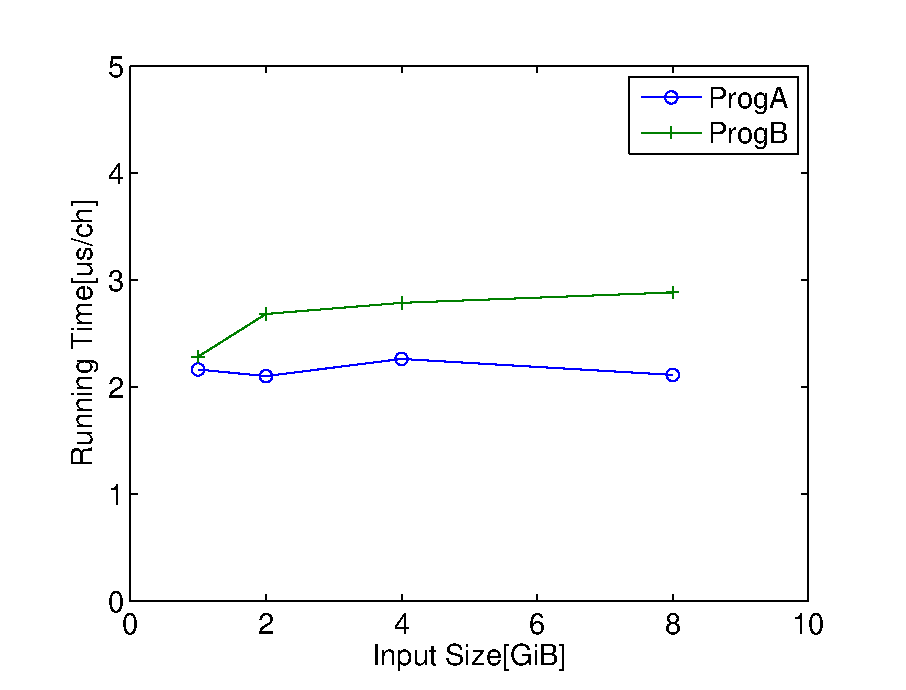
\includegraphics[width = 0.8\columnwidth]{ct_cmp2}
	}
	\caption{Experimental results for prefixes of "enwiki".}
	\label{fig:performance_analysis2}
\end{figure}
	
	\subsection{Discussion}
	
	It is identified that both programs heavily rely on the performance of the external memory sorter in use. A potential candidate for improving their speed is to adapt a GPU-based multi-way sorter~(e.g.,~\cite{Leischner2010, Davidson2012}) for sorting massive data using external memory. By the aid of these fast sorting algorithms, the throughputs of the programs are expected to nearly approach the I/O bandwidth. Besides, the first two steps of Algorithm~\ref{alg:1} are independent of each other and thus can be executed in parallel for acceleration. This technique can be also applied to check the suffix and LCP arrays of the LMS suffixes in Algorithm~\ref{alg:3}.
	
	Currently, for Algorithm~\ref{alg:3}, step 2 constitutes the space bottleneck. It is worthy of mentioning that this step produces a copy of the suffix and LCP array during the inducing and checking processes. Actually, given that $\Sigma$ is of a constant size and $sa/lcp$ are known already, we can simply scan the input $sa/lcp$ to perform the inducing process and compare each induced suffix/LCP value with that in the given $sa/lcp$ to perform the checking process, resulting in less space consumption. To the end, we must maintain a read pointer for each suffix/LCP bucket in $sa/lcp$ to scan elements in sequence.
	
\section{Conclusions} \label{sec:conclusion}

In this article, we propose two methods for probablistically checking the give suffix and LCP arrays using external memory. According to the experimental results, our program for Method A has a better performance than that for Method B with respect to the running time and I/O volume by about 20 percent, while the peak disk use of the latter is about 26/40=0.65 as that of the former and can be further reduced to around 21n without a sacrifice in the time and I/O effciency. We think these two methods could potentially be a xxxx .	 




% Bibliography
\bibliographystyle{IEEEtran}
\bibliography{IEEEabrv,bibfile}
	
\end{document}


We are intended for ....

put emphasis on

with the same ease as when

The biggest difference between two is that ...

Toward the end, ...

they are designed to be both easy to interpret on ... and easily traslated into ... (they are designed to be easily implemented in classic external memory models)

Having a ... eliminates .... (random accesses), access ordering

Not only are ..., but 

The fingerprints are calculated on the fly during the scan of x ...

become so good that they are competitive with ...., and in some cases, even outperform them ...

concurrent programming is needed to make sure ....

designed to adapt to an evolving environment

most importantly

exchanges data between the computer presenting the applet and the computer serving it.

carries out sophisticated calculations

Presumably because

make ... capable of ...

greatly improve ... , it was still rather limited, though.


additional performance improvements

close the chapter with ...

gain

which pose ...

integrate with

In this chapter, we will ... how to ... and how to ...


we prefer the comfort of an integrated development environment, ( prefer the low cost of fingerprinting techinques)

space-hungry


begin exploring ... by ...

commnuicate the monmentous advances

extremely simple

check each number is present in the suffix array.

go into much more greater details

stand-alone algorithms for computing suffix arrays only and has been reused to 

invoke/call


the mechanics of ...

If you have done sth, then when you do sth, you end up with ...

depend on the machine on which you will be running the java code ...


alleviate



The second method is invented to overcome the drawback of 

in place of

as to/about

as far as

assign to a variable

stated goals

intermediate steps

tied to the behavior of 

an assortment of 

following the footsteps of 

characters in the input string are processed from left to right

in greater detail




































